\section{Experimental setup}
\label{sec:setup}
\paragraph{Benchmark and adaptation.}
We evaluate the official RoboMME test split: 16 tasks across Counting, Permanence, Reference, and Imitation, with 50 episodes per task and 800 in total \citepending{robomme}. Episode seeds and difficulty follow the benchmark specification; official environment feedback determines success. We use GPT-6 Astra as the supervisor and the official RoboMME GroundSG checkpoint, a grounded-subgoal \pifive\ policy, as the VLA. The VLA weights remain fixed. Initial experience consists of duration recommendations derived from subtask completion-step statistics in training demonstrations. In every task, the first five episodes permit experience updates after either outcome; the remaining 45 permit updates only after unsuccessful outcomes. All 50 episodes contribute to the reported success rate. The experience store remains fixed within each episode, and accepted revisions are made available to subsequent episodes. Appendix~\ref{app:configuration} specifies model settings, limits, and cross-task sharing.

\paragraph{Observation access.}
The harness uses the task instruction, front and wrist RGB images, and robot state available to the VLA under standard RoboMME evaluation. Historical observations come from the same observation stream. Planning and control receive no privileged environment ground truth, such as hidden object states or oracle subgoals. Official success and termination feedback is used for outcome assessment and post-episode review.

\paragraph{Comparisons.}
Table~\ref{tab:performance} groups learned policies, direct VLM control, and hierarchical systems, reporting overall success \citepending{robomme,memer,simplememvla,astra-direct,ponderpounce,astra-three-tier}. Human skill selection and GroundSG+Oracle are separate privileged references. PonderPounce-9B uses the reported standard-data leaderboard result, and the other reference scores follow the cited benchmark and system reports; controller training, history access, intervention interfaces, and test-time experience updates differ across systems. We additionally compare delegation with per-chunk review on ten StopCube test seeds. Both conditions are rerun with the same models, history tools, recovery interfaces, and execution limits. Within each pair, both read the same saved version of the experience store, and experience updates are disabled. Runs are serial, with the order of conditions alternating across pairs. This comparison isolates review policy under a fixed experience context for each seed.

\paragraph{Measurements.}
We report task success and the distribution of control steps across four execution modes: subgoal entry, Astra intervention, automatic VLA continuation, and VLA continuation after review. The last mode is the first VLA chunk released after Astra checks progress on the current subgoal; subsequent chunks within the same budget count as automatic continuation. Completion time includes model inference, history queries, action execution, and waiting. Completion-time statistics are reported for successful episodes, since failed runs may terminate early or continue until the execution limit. Appendix~\ref{app:measurements} gives detailed accounting.

\section{Results and analysis}
\label{sec:results}
\subsection{Task performance}
The harness succeeds in 777 of 800 episodes (97.1\%; Table~\ref{tab:performance}), exceeding the published direct-Astra and three-tier Astra scores by 5.0 and 18.0 percentage points, respectively. Success reaches 97.0\% on Counting, 97.5\% on Permanence, and 97.0\% on both Reference and Imitation. Every task achieves at least 90\%, and seven reach 50/50 successes. Gains over direct Astra are particularly large on MoveCube (100\% versus 54\%) and StopCube (96\% versus 54\%). The task results in Figure~\ref{fig:task-comparison} show that the combined system performs well across all four memory categories.

\begin{figure}[!htbp]
\centering
\captionsetup{font=small,justification=raggedright,singlelinecheck=false}
\begin{minipage}[t]{0.37\linewidth}
\vspace{0pt}
\captionof{table}{Overall success on RoboMME (\%).}
\label{tab:performance}
\small
\setlength{\tabcolsep}{4pt}
\renewcommand{\arraystretch}{1.08}
\begin{tabularx}{\linewidth}{@{}Xr@{}}
\toprule
\textbf{Method} & \textbf{Overall} \\
\midrule
\rowcolor{ink!7}\multicolumn{2}{l}{\footnotesize\bfseries Learned policies} \\
\hspace{3pt}\pifive & 17.9 \\
\hspace{3pt}FrameSamp+Modul & 44.5 \\
\hspace{3pt}SAM2Act+ & 21.4 \\
\hspace{3pt}SimpleMemVLA & 88.3 \\
\addlinespace[3pt]
\rowcolor{ink!7}\multicolumn{2}{l}{\footnotesize\bfseries Direct VLM control} \\
\hspace{3pt}Astra & 92.1 \\
\addlinespace[3pt]
\rowcolor{ink!7}\multicolumn{2}{l}{\footnotesize\bfseries Hierarchical systems} \\
\hspace{3pt}MemER & 42.4 \\
\hspace{3pt}GroundSG+QwenVL & 32.7 \\
\hspace{3pt}GroundSG+Gemini & 11.6 \\
\hspace{3pt}PonderPounce-9B & 60.8 \\
\hspace{3pt}Three-tier Astra & 79.1 \\
\rowcolor{blue!7}\hspace{3pt}\textcolor{blue!65!black}{\textbf{Our harness}} & \textbf{97.1} \\
\addlinespace[3pt]
\rowcolor{ink!7}\multicolumn{2}{l}{\footnotesize\bfseries Privileged references} \\
\hspace{3pt}Human & 90.5 \\
\hspace{3pt}GroundSG+Oracle & 84.1 \\
\bottomrule
\end{tabularx}
\end{minipage}\hfill
\begin{minipage}[t]{0.60\linewidth}
\vspace{0pt}
\centering
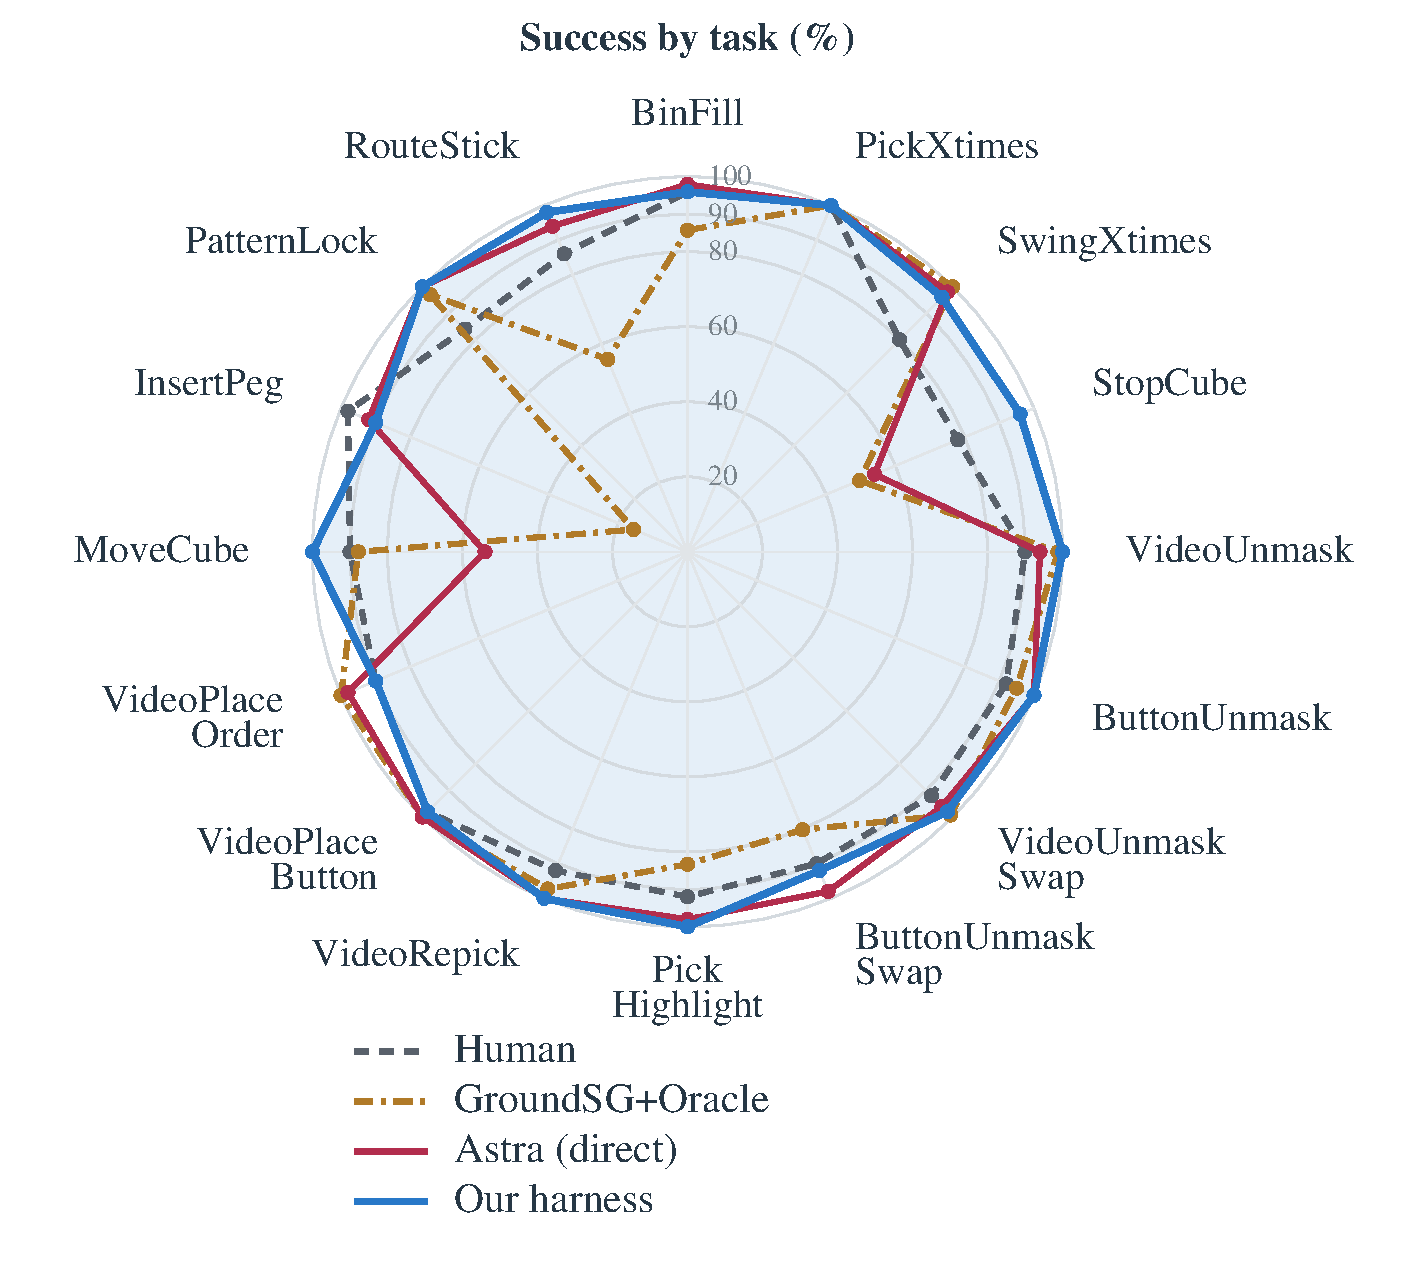
\includegraphics[width=\linewidth]{task_comparison.pdf}
\captionof{figure}{Per-task success of our harness and published references \citepending{robomme,astra-direct}. Human uses an oracle skill interface; GroundSG+Oracle supplies true subgoals to a learned policy; Astra directly specifies waypoints.}
\label{fig:task-comparison}
\end{minipage}
\end{figure}

\FloatBarrier
\subsection{Supervision and execution efficiency}
Automatic VLA continuation accounts for 54.93\% of control steps, allowing more than half of execution to proceed without additional Astra review (Table~\ref{tab:allocation}). Astra intervenes directly in 33.5\% of episodes, but these interventions account for only 4.91\% of control steps. Most motion therefore remains with the learned controller, while Astra contributes local corrections when needed.

\begin{table}[!htbp]
\centering
\caption{Distribution of executed control steps across 800 episodes. Automatic continuation proceeds without an additional Astra review.}
\label{tab:allocation}
\small
\begin{tabularx}{0.85\linewidth}{@{}Xr@{}}
\toprule
Execution mode & Control steps (\%) \\
\midrule
Subgoal entry & 17.23 \\
Astra intervention & 4.91 \\
Automatic VLA continuation & 54.93 \\
VLA continuation after review & 22.93 \\
\bottomrule
\end{tabularx}
\end{table}

Review frequency adapts to the demands of each task. Insertion involves error-prone contact and alignment, so InsertPeg often requires close inspection and corrective action. RouteStick instead contains short directional subtasks; Astra tends to permit one chunk at a time to avoid continuing past a subtask boundary. In VideoPlaceButton, Astra can allow longer execution intervals once the target has been identified. These patterns suggest that review needs vary across task stages, with some stages requiring closer supervision than others.

Appendix~\ref{app:completion-time} reports full-benchmark completion times. We use a matched comparison to examine the effect of review frequency on execution time and model usage.

\paragraph{Matched review-policy comparison.}
Delegation reduces completion time on the nine StopCube seeds that succeed under both review policies (Table~\ref{tab:paired}). Mean execution time falls from 513.2 to 285.6\,s, a reduction of 44.3\%, and delegation is faster in all nine pairs. Across all ten seeds, the two conditions execute similar numbers of control steps, while delegation automatically continues 57.6\% of execution requests and reduces total input tokens by 60.7\%. Per-chunk review succeeds on 10/10 seeds and delegation on 9/10. This comparison shows that delegation can substantially reduce execution time and token usage, although it fails on one seed completed successfully by per-chunk review.

\begin{table}[!htbp]
\centering
\caption{StopCube review-policy comparison on ten matched seeds with experience updates disabled. Timing uses successful episodes; the paired row uses the nine seeds successful in both conditions. Token counts include cached input and cover execution across all ten episodes.}
\label{tab:paired}
\small
\begin{tabularx}{\linewidth}{@{}Xrr@{}}
\toprule
Measurement & Per-chunk review & Delegation \\
\midrule
Successes / episodes & 10/10 & 9/10 \\
Successful episodes: mean time (s) & 512.0 & 285.6 \\
Successful episodes: median / P90 (s) & 548.8 / 727.0 & 240.2 / 392.0 \\
Jointly successful seeds: mean time (s) & 513.2 & 285.6 \\
Automatic / all requests (\%) & 0.0 & 57.6 \\
Mean control steps / episode & 202.1 & 201.0 \\
Total input tokens (millions) & 30.63 & 12.05 \\
Uncached input tokens (millions) & 2.22 & 1.19 \\
\bottomrule
\end{tabularx}
\end{table}

\FloatBarrier
\subsection{Execution and experience analysis}
Across the evaluation, Astra updates the experience store after 37 episodes, producing 43 entries, including seven revisions of earlier advice. Later execution decisions explicitly cite 38 of these entries across 468 episodes. The cases below show how this reused experience changes review intervals and target interpretation, helping Astra adapt its supervision to the VLA's observed behavior.

\paragraph{Revising execution advice.}
In PickXtimes, Astra observes hovering during button pressing and subsequently adds a stationary-motion monitor to the recommended 90-step budget. In the next episode, execution again reaches the 90-step budget without triggering the monitor. The recorded motion never satisfies the 2\,mm stationary threshold over a 32-step window: the smallest position diameter is 26.9\,mm. Astra revises the advice to 60 initial steps, with review intervals of at most 16 steps during contact or recovery. In the following episode, Astra explicitly cites the revision and sets a 60-step budget with the stationary-motion monitor enabled. The VLA executes four chunks of 16, 16, 16, and 12 steps before budget exhaustion; Astra then permits another action chunk, which completes the task after 13 steps. Figure~\ref{fig:trace} illustrates this revision and subsequent execution. The revised advice brings visual review forward while retaining stationary-motion monitoring as another way to trigger review.

\begin{figure}[!t]
\centering
\captionsetup{font=small}
\caseframe{PickXtimes-ep0-f689}{\textbf{Episode 0} / frame 689}{Hovering inspected after execution}\hfill
\caseframe{PickXtimes-ep1-f284}{\textbf{Episode 1} / frame 284}{90-step budget; monitor does not trigger}\hfill
\caseframe{PickXtimes-ep2-f288}{\textbf{Episode 2} / frame 288}{Review after the revised 60-step budget}
\caption{Experience revision across three PickXtimes episodes. Hovering motivates adding a stationary-motion monitor; continued motion prevents it from triggering in episode 1. Astra then shortens the budget from 90 to 60 steps and adopts this advice in episode 2. Figure~\ref{fig:within-episode-cases}(a) follows episode 2 from review to completion.}
\label{fig:trace}
\end{figure}

\paragraph{Revising historical interpretation.}
In VideoPlaceButton, a failed episode leads to advice for tracking visually similar rings through late demonstration swaps, but the resulting recommendation incorrectly assumes a before-press query. In the next episode, the task asks for the first event after the press; Astra recognizes that the earlier rule does not apply and subsequently revises it to condition on the current temporal query. A later episode asks for the last event before the press. Astra explicitly cites the revision in its notes and execution decision, examines the relevant historical frames, and selects the topmost ring. With an 80-step budget, the VLA completes the task after 54 steps. The revision preserves the identity-tracking advice while making target selection conditional on the requested temporal relation (Figure~\ref{fig:history-case}).

\begin{casefigure}
\caseframe{VideoPlaceButton-ep3-f700}{\textbf{Episode 3} / frame 700}{Late swap inspected after failure}\hfill
\caseframe{VideoPlaceButton-ep4-f501}{\textbf{Episode 4} / frame 501}{First-after query exposes the rule's limit}\hfill
\caseframe{VideoPlaceButton-ep10-f1006}{\textbf{Episode 10} / frame 1006}{Revised rule used for a last-before query}
\caption{Experience revision across three VideoPlaceButton episodes. The first rule tracks ring identity but assumes a before-press query. A first-after query prompts a conditional revision, later applied to a last-before query. Figure~\ref{fig:within-episode-cases}(b) shows the late swap within episode 3.}
\label{fig:history-case}
\end{casefigure}

\subsection{Failure analysis}
We manually inspect all 23 failed episodes and group their primary causes into historical interpretation (8), subgoal grounding (1), execution (9), and review or recovery (5).

Specifically, historical interpretation accounts for all five VideoPlaceOrder failures and also affects VideoPlaceButton and InsertPeg. The RouteStick grounding error concerns the task's left--right convention. Execution problems include insufficient endpoint motion in two SwingXtimes episodes and insufficient container lift in one VideoUnmaskSwap episode. Two ButtonUnmaskSwap episodes advance before the button action is complete, and the two StopCube failures involve early or missed button timing. Repeated alignment and contact recovery also leave some InsertPeg episodes unsuccessful. These cases identify where history interpretation, progress review, and local correction still need improvement; representative trajectories appear in Figure~\ref{fig:failures}, with further details in Appendix~\ref{app:failure-analysis}.
